
\documentclass[12pt]{rutgersthesis}

% preamble

% Make sure your LaTeX files are put under the root of your work directory. They should not be in a subfolder!

%%%%%%%%%%%%%%%%%%%%%%%%%%%%%%%%%%%
% Your information here
% !IMPORTANT!
%%%%%%%%%%%%%%%%%%%%%%%%%%%%%%%%%%%
\newcommand{\thesisType}{Dissertation} % Dissertation for PhD and Thesis for Master
\newcommand{\thesisTitle}{Title} % your thesis/dissertation title, e.g., How to Write A Thesis
\newcommand{\yourName}{Name} % your name, e.g., Tim Cook
\newcommand{\yourDegree}{Doctor of Philosophy} % your degree to be obtained, e.g., Master of Science, Doctor of Philosophy
\newcommand{\yourProgram}{Graduate Program} %insert your graduate program’s official name
\newcommand{\yourDirectorTitle}{Prof.} % the title of your thesis director
\newcommand{\yourDirector}{Dissertation/Thesis Director} % your thesis director name here, his/her title not included
\newcommand{\yourCommitteeNumber}{4} % IMPORTANT! the number of the committee members for your defense
\newcommand{\yourMonth}{Month} % your graduation month, not your defense month
\newcommand{\yourYear}{Year} % your graduation year


\bibliography{references}

% document body
\begin{document}
% \doublespacing  %set line spacing

\clearpage
\begin{center}

\vspace*{\fill}

\copyright { }{\yourYear}\\
{\yourName}\\
ALL RIGHTS RESERVED\\

\vspace*{\fill}

\end{center}

\pagenumbering{gobble}
\clearpage

\makeTitlePage{Month}{Year}

\begin{frontmatter}
    \begin{my_abstract}

Abstract. 

\end{my_abstract}
    
\begin{acknowledgments}

Acknowledgments.

Acknowledgment of previous publications \labelcref{pubs:P1}.

\end{acknowledgments}

    \makeTOC
    \makeListOfTables
    \makeListOfFigures
    %
\newacronym{starlabs}{STAR Labs}{Scientific and Technological Advanced Research Laboratories}
\newacronym{uv}{UV}{ultraviolet}

\makeListOfAcronyms
\end{frontmatter}

\begin{thesisbody}
    
\chapter{Introduction and Background}
\thispagestyle{myheadings}

\section{Stars}

It is common knowledge that the star closest to Earth is the Sun, and also that the Sun is yellow. It is this yellow sunlight which is interesting for some of its properties \cite{scholes2011lessons}. For instance, plants, algae, and cyanobacteria convert this light into energy via photosynthesis. In \ref{fig:firstFig} is a photo of a galaxy which contains many stars.

\begin{figure}[ht]
    \centering
	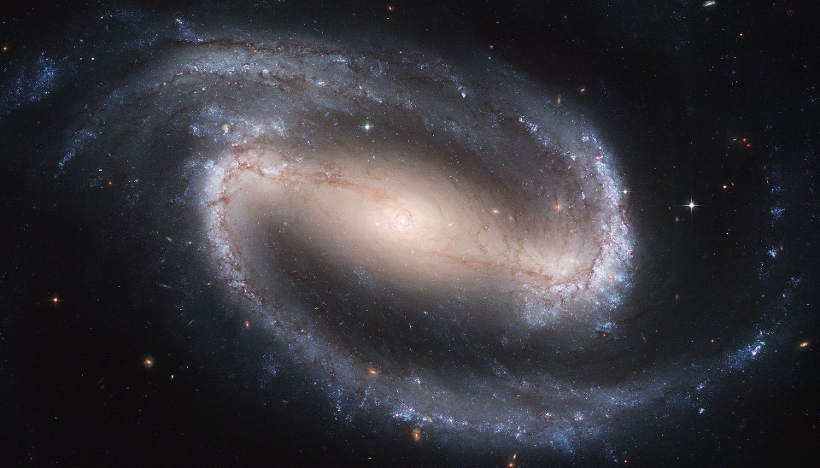
\includegraphics[width=0.85\textwidth]{figures/sampleFig1.jpg}
	\caption[Barred spiral galaxy NGC 1300]{Barred spiral galaxy NGC 1300 photographed by Hubble telescope. While the galaxy in the photo is not our sun, it does emit light, much like our sun. Image credit: NASA.}
	\label{fig:firstFig}
\end{figure}

The stars in the sky are of particular interest to the aptly named \gls{starlabs}, which in many recent experiments has shown promising results in converting this energy in a non-photoelectric sense into usable energy \cite{allen2019fast}. Interestingly, \gls{starlabs} has theorized that the famous superhero known as ``Superman'' converts the light from our sun, which grants his fantastic abilities. There are many methods in industry for converting the sun's energy (of about \SI{1000}{\watt\per\meter\squared}) into electrical energy. Some of these are highlighted in \ref{tbl:sampleTbl1}.

\begin{table}[ht]
\centering
\caption[Selected renewable energy installations]{Renewable energy installations around the world -- the energy generated at these sites is ultimately derived from the sun}
\label{tbl:sampleTbl1}
\resizebox{0.8\textwidth}{!}{%
\begin{tabular}{llll}
\hline
installation & type & capacity (GW) & location \\ \hline
Longyangxia Dam & photovoltaic & 0.85 & China \\
Gansu Wind Farm & wind & 6 & China \\
Sihwa Lake & tidal & 0.254 & South Korea \\ \hline
\end{tabular}%
}
\end{table}
    
\chapter{Methodology}
\thispagestyle{myheadings}

The process of data collection began with analysis of the physical principles underlying optical light emission.

\section{The Various Types of Light}

Depending on the energy of a photon, it may be referred to as ``light'' (in the case of optical photons) or as something else -- for example, a gamma ray. By convention, there are many names for these particles.

\subsection{Low-energy photons}

The lowest energy electromagnetic radiation is carried by radio waves.

\subsection{Intermediate-energy photons}

These include several types of radiation, including the usually-harmful \gls{uv}.

\subsubsection{Microwaves}

Microwaves have wavelengths on the order of \SI{1e-2}{\meter}, or a few \si{\centi\meter}.

\subsubsection{Visible light}

Visible light is that which is detectable by the human eye, with wavelengths about \SIrange{380}{750}{\nano\meter}.


    % 
\chapter{Results}
\thispagestyle{myheadings}

% text of this chapter goes here
    % 
\chapter{Discussion}
\thispagestyle{myheadings}

% text of this chapter goes here
    % 
\chapter{Conclusion}
\thispagestyle{myheadings}

% text of this chapter goes here

    \begin{publications}
\thispagestyle{myheadings}

%% Please use \labelcref instead of \ref when refer to your publications!

\begin{enumerate}[leftmargin=*,start=1,label=\textbf{P\arabic*}, ref={P\arabic*}]
    \item \label{pubs:P1} Publication 1.
    \item \label{pubs:P2} Publication 2.
    \item \label{pubs:P3} Publication 3.
\end{enumerate}

\end{publications}

    \makeBibliography
    
\begin{theappendices}
    \chapter{Experimental Equipment}
    \thispagestyle{myheadings}
    A telescope and a spectrometer were used to analyze the sun. Many other instruments were used.
    
    \chapter{Data Processing}
    \thispagestyle{myheadings}
    Data was processed before being added to this document.
    
\end{theappendices}
\end{thesisbody}

\end{document}
